\documentclass[review]{elsarticle}
\usepackage{lineno,hyperref}
\modulolinenumbers[5]
\usepackage[margin=1in]{geometry}
\usepackage{graphicx}
\usepackage{placeins}
\usepackage{comment}

\bibliographystyle{elsarticle-num}

\begin{document}
\begin{frontmatter}
\title{First principles study of Nd energetics and diffusion in $\alpha$ U}

\author[inl]{Benjamin Beeler\corref{qwe}}
\cortext[qwe]{Corresponding author}
\ead{benjamin.beeler@inl.gov}
\author[inl]{Yongfeng Zhang}
\address[inl]{Idaho National Laboratory, Idaho Falls, ID 83415}


\begin{abstract}

\end{abstract}
\end{frontmatter}

\linenumbers

\section{Introduction}

Uranium-zirconium (U-Zr) and uranium-plutonium-zirconium (U-Pu-Zr) alloy fuels have a history of usage in sodium-cooled fast reactors. Not only does the U-Zr fuel (as well as U-Pu-Zr) generate a harder neutron spectrum as compared to traditional ceramic fuels, but it also offers excellent neutron economy and high burnup capability \cite{hofman1997}. Recently, U-Zr fuels have regained interest due to the possibility of incorporating minor actinides into the fuel, and as such the metallic fuel alloys would serve to reduce the quantity of long-lived radioisotopes present in nuclear waste \cite{capriotti2017}. 

One issue with metallic fuels, including both UZr and UMo fuels, is the large amount of swelling that takes place \cite{hofman1997}. Such swelling can be accounted for in the fuel design, however the swelling needs to be stable and predictable up to high fission densities. As shown in Fig. \ref{fig:ben1}, research reactor fuel types based on UMo are unique in that there cannot exist fission gas release from the fuel, and as such there is a relatively high content of fission gas and of fission gas bubbles within the fuel matrix. This importance of swelling in addition to the unique fuel environment has led to a variety of studies attempting to characterize the swelling behavior in U-Mo fuels \cite{rest2009, kim_anl08, meyer2002, kim2013} which has led to the development of a swelling correlation from Argonne National Labortory (ANL correlation) \cite{kim2011} as a function of fission density. This swelling correlation was intended to be applicable for low temperature (less than 250$^{\circ}$C) U-Mo alloys in the 7-10 wt.\% composition range. 

U-Zr alloys are typically employed as a series of fuel pellets within a given fuel rod, similar to UO$_{2}$ fuels. Unlike UO$_{2}$ fuels, dramatic swelling is inevitable, and is typically accounted for by manufacturing fuels with a smear density of approximately 75{\%}. This allows for approximately 30\% swelling, which is sufficient to allow fission gas release \cite{beck1968}. The nature of swelling is anisotropic in these fuels, largely due to the difference in swelling behavior between the hotter center of the fuel and the colder periphery \cite{hofman1990}. The degree of anisotropicity increases with increasing Pu content. During operation, the phenomenon of constituent redistribution takes place. This results in three distinct radial regions within the fuel. The innermost region is Zr-rich, the intermediate region is Zr-poor and the outermost region has a nominal Zr concentration. This phenomenon is due to both the effect of the temperature gradient on phase equilibria and the diffusion of species along the temperature gradient. This concentration variance as a function of radius in combination with the temperature gradient leads to the $\gamma$ phase being present in the interior of the fuel pellet, while the $\alpha$ phase predominates the periphery \cite{kobayashi1990, kim2004}. The radially anisotropic swelling within the fuel pellet is due to the variation in phases as a function of radius.


WIRTH TEXT
$Metallic fuels are ideal for fast (breeder) reactors because they produce an extremely hard neutron spectrum. U-Zr and U-Pu-Zr alloys are two important potential metallic fuels for fast reactors. However, the swelling of metallic fuels is much more severe than for mixed-oxide fuel, and is an important issue for metallic fuels. Fission product gas (Xe, Kr) bubble growth is believed to be responsible for the swelling. Computational modeling of gas bubble nucleation and growth is useful for predicting and ultimately developing mitigation strategies for the swelling behavior of the fuel. The formation energy and migration barrier of vacancy, interstitial and gas atoms (Xe, Kr) are fundamental parameters of the computational model. However, they are very difficult to obtain from experiments, and not available in the literature to date. Diffusion experiments can provide information on atomic migration and, in addition, allow one to gain insights into the defect chemistry. However, these data are deficient at present. As an example, the available experiment results in the literature are for pure ? uranium, but not for ? U?Zr.  Thus the influence of Zr is not clear. In addition, there are no available experiment results for interstitial behavior. Similarly, although the activation energy of self-diffusion can be obtained from experiments, the formation energy, migration barrier and diffusion mechanisms are difficult to confirm in experiments, and not available in the literature. Finally, it is very difficult to fabricate ?perfect? single crystals of uranium metal in experiments and not easy to perform diffusion experiments for uranium, due to the nature of uranium. Based on first principles calculations, the formation energy and migration barrier of vacancy and interstitial defects, and the influence of Zr on these values, can be obtained and compared with experimental results. The calculations of point defects, and later Xe, in U?Zr alloys will provide a foundation for computational modeling of fission gas bubble nucleation and growth. Although ? U has been extensively investigated by first-principles methods [1?17], information on interstitial and vacancy diffusion is still deficient. It is necessary to pursue further studies to understand the diffusion behaviors of the interstitial and vacancy in systematic research.  In the outer zone of U?Zr metallic fuel, the dominant microstructure consists of an ? phase matrix with ?-lamellae [18]. Due to the lower temperature, the bubble nucleation and growth are more severe. In this paper, we will focus on the ? phase of U?Zr alloys. The structure of ? uranium is made up of close-packed corrugated layers of atoms, with layers parallel to the (010) plane and the corrugations parallel to the [100] axis. The self-diffusion along the [010] direction is believed to be much more difficult than in the other two directions [19]. The activation energy of self-diffusion in pure uranium along all three principal directions has been obtained experimentally and is reported as 1.91 eV [20] along the [100] and [001] directions, and 2.91 eV [21] along the [010] directions. The corrugated structure does not affect the diffusion parallel to the (010) plane significantly. As illustrated in [21], the measurement of the diffusion coefficient along the [010] direction is more difficult than for the other two directions. There is only one report in the literature for the [010] direction, and no experiment details are available [21]. For the [100] and [001] directions, there are more reports in the literature, and more experiment details are available [20]. There are only two data values reported for ?perfect? single crystals in the literature for the [100] and [001] directions, from two different authors. Using these two data points to fit an Arrhenius equation results in an activation energy of about 2.3 eV [20]. However, based on only these two data values from two different authors, it cannot be fully considered as an accurate value. Therefore, the activation energy (1.91 eV) along the [100] and [001] directions is obtained using the data of a so-called ?single crystal with mosaic structure? [20]. It should be smaller than the actual value due to the mosaic structure of the sample. Additionally, there are three other activation energy values reported in the literature (1.99 eV [22, 23], 2.15 eV [24, 25] and 2.21 eV [26, 27]), which do not specify the direction. All of these values are within the range 1.91?2.91 eV. Therein, only 1.99 eV is reported with the Arrhenius diagram [22, 23].  It is likely that these three values are for the [100] and [001] directions, due to the difficulty of measurement for the [010] direction; the original literature is not accessible. We note that the activation energy in polycrystal uranium (1.74 eV [20, 28]) tends to be smaller than in single-crystal uranium (1.91? 2.91 eV). On the other hand, diffusion of interstitial via an interstitial mechanism or interstitialcy mechanism (kick-out mechanism) is proposed to be nearly isotropic, which is seldom investigated in the literature [29].  No experimental results of interstitial in pure uranium is available. In some simulations reported in the literature, the migration barrier is assumed to be 0.15 eV [30]. Formation energy of the vacancy in pure ? uranium is difficult to obtain by experiment, and was calculated by Taylor [9] (1.95 eV) and Beeler [17] (1.86 eV) with first-principles methods. However, both of them suffer from unexpected problems, as discussed in section 2.  Based on our first-principles calculations, the formation energy of the vacancy in pure ? uranium is 1.69 eV. The diffusion of vacancy is almost isotropic in the [100] and [001] directions, 0.34 eV and 0.36 eV, respectively, and 1.24 eV for the [010] direction. The corresponding activation energy of self-diffusion is thus 2.03 eV along the [100] direction, 2.05 eV along the [001] direction and 2.93 eV along the [010] direction.  Compared with the experimental results, the activation energy along the [100] and [001] directions (2.03 and 2.05 eV) is about 0.1 eV larger than the experimental results (1.91 eV), and the activation energy along the [010] direction (2.93 eV) agrees very well with experimental results (2.91 eV). Given that 1.91 eV is actually for a single crystal with mosaic structure, and the results of ?perfect? single crystals tend to have larger activation and smaller diffusion coefficient, the deviation can be understood. Of course, more experimental data are needed to fully resolve the inconsistency and validate the first-principles calculation results.  At 612 ?C, the equilibrium concentration of Zr in ? U is about 0.5$\%$ according to the phase diagram [31]. The presence of Zr would influence the formation energy and migration barrier of intrinsic point defects significantly. However, to date, very little information is available in the literature. In order to investigate the influence of Zr, we focus on the binding energy between the vacancy and Zr, the dissociation barrier of the vacancy from Zr, and the rotation barrier of the vacancy around Zr.$
WIRTH TEXT

\section{Computational Details}
Systems are investigated using the Vienna $\textit{ab initio}$ Simulation Package (VASP) \cite{vasp1, vasp2, vasp3, vasp4}.  The projector augmented wave (PAW) method \cite{paw1, paw2} is utilized within density functional theory \cite{dft1, dft2}.  Calculations are performed using the Perdew-Burke-Ernzerhof (PBE) \cite{pbe1, pbe2} generalized gradient approximation (GGA) for the description of the exchange-correlation.  Methfessel and Paxton's smearing method \cite{methfessel} of the first order is used with a width of 0.1 eV to determine partial occupancies for each wavefunction.  Wavefunction optimization was truncated when the energy difference was less than 10$^{-5}$ eV.  The optimization procedure was truncated when the residual forces for the relaxed atoms were less than 0.01 eV/{\AA}.  Symmetry is switched off for all calculations.  A support grid is utilized for the evaluation of augmentation charges.  Non-spherical contributions from the gradient corrections inside the PAW spheres are included.  Convergence testing was performed for this system in the model of Huang and Wirth \cite{wirth2011} (utilized Perdew-Wang (PW91) \cite{pw91, pw91b} GGA).   The energy cutoff is increased, the supercell is increased in size, and the k-points mesh is refined until the energy of the pure system and the formation energy of a vacancy vary by less than 5 meV.  The convergence testing led to the choice of a 252 atom supercell (7x3x3 unit cells), a cutoff energy of 400 eV and a gamma-centered k-points mesh of 4x2x4, resulting in 20 k-points in the irreducible part of the Brillouin zone. The calculated lattice parameters are $\it{a}$ = 2.803 {\AA}, $\it{b}$ = 5.836 {\AA}, $\it{c}$ = 4.906 {\AA} and $\it{y}$ = 0.098.  These results compare very favorable to previous results \cite{wirth2011, soderlind2002, taylor2008}  and experiments \cite{barrett1963}.  

In order to obtain migration barriers for the various pathways investigated, we utilized the climbing-image nudged elastic band (CI-NEB) method \cite{neb1}.  Both single and multiple image implementations of the CI-NEB method were implemented to ensure that both the correct migration pathway and the correct migration barrier magnitude were obtained. 

\section{Results}

\subsection{Defect formation energies in $\alpha$U}

To verify the methodologies presented in this study, the formation energy of a single vacancy and a single interstitial in $\alpha$U were calculated utilizing equation \ref{eqn:vac} and \ref{eqn:int}, respectively,

\begin{equation}
\label{eqn:vac}
E_{f}^{vac} = E_{vac} - (n-1)*E_{pure}
\end{equation} 

\begin{equation}
\label{eqn:int}
E_{f}^{int} = E_{int} - (n+1)*E_{pure}
\end{equation} 

where E$_{vac}$ is the total energy of the system with a vacancy, E$_{int}$ is the total energy of the system with an interstitial, E$_{pure}$ is the energy per atom of a defect-free system, and \textit{n} is the number of atoms in the defect-free system. The vacancy formation energy is calculated to be 1.70 eV, which compares very favorably with the calculations of Huang and Wirth \cite{wirth2011} (1.69 eV).  

Nd interstitial 7.8 eV.  A Nd substitutional of 2.106 eV and U interstitial of 4.31 eV \cite{wirth2012} have a lower combined energy than the Nd interstitial.  Thus it would be expected that if a Nd interstitial is created, it would transform into a substitutional Nd atom and create a U SIA.  Therefore, only vacancy-mediated diffusion of Nd atoms is investigated.  Also, vacancy migration in the corrugated plane in four time as likely (migration barriers of 1.24 eV out of corrugated plane, 0.36 eV and 0.34 eV in corrugated plane \cite{wirth2011}, thus only vacancy migration in the corrugated plane is investigated.  

\begin{table}[h!]
\caption{Formation energies for vacancy-Nd defects in alpha U.}
\label{tab:Eforms}
\begin{center}
\begin{tabular}{|c|c|}
     \hline
      Defect & E$_{form}$  \\
     \hline
     vacancy & 1.701  \\
     Nd sub & 2.106 \\
     Nd Vac X & 2.886 \\
     Nd Vac Z & 2.627 \\
       \hline
\end{tabular}
\end{center}
\label{default}
\end{table}%

Needs Nd-vac binding energies??

\begin{table}[h!]
\caption{Formation energies of multi-vacancy defect complexes in alpha U}
\label{tab:Eforms}
\begin{center}
\begin{tabular}{|c|c|}
     \hline
      Defect & E$_{form}$  \\
     \hline
     Divac X & 3.835 \\
     Divac Z & 3.638 \\
     Divac 2nn X & 3.377 \\
     Divac 2nn Z & 3.616 \\
     Nd Divac X & 4.845 \\
     Nd Divac Z & 4.161 \\
     Nd Divac XZ & 4.081 \\
     Trivac X & 5.858\\
     Trivac Z & 5.553 \\
     Trivac XZ & 5.549 \\
       \hline
\end{tabular}
\end{center}
\label{default}
\end{table}%

\begin{table}[h!]
\caption{Formation energies of Nd and Pd point defects in alpha U.}
\label{tab:Eforms}
\begin{center}
\begin{tabular}{|c|c|}
     \hline
      Defect & E$_{form}$  \\
     \hline
     Pd sub & 0.218 \\
     NdPd X &  -1.709 \\
     NdPd Z & -1.705 \\
     Pd Vac X & 1.693 \\
     Pd Vac Z & 1.627 \\
       \hline
\end{tabular}
\end{center}
\label{default}
\end{table}%


Nd with vac Z -  sits slightly off of lattice site, as shown in Figure \ref{fig:ndvacz}.

\begin{figure}[ht]
	\centering
	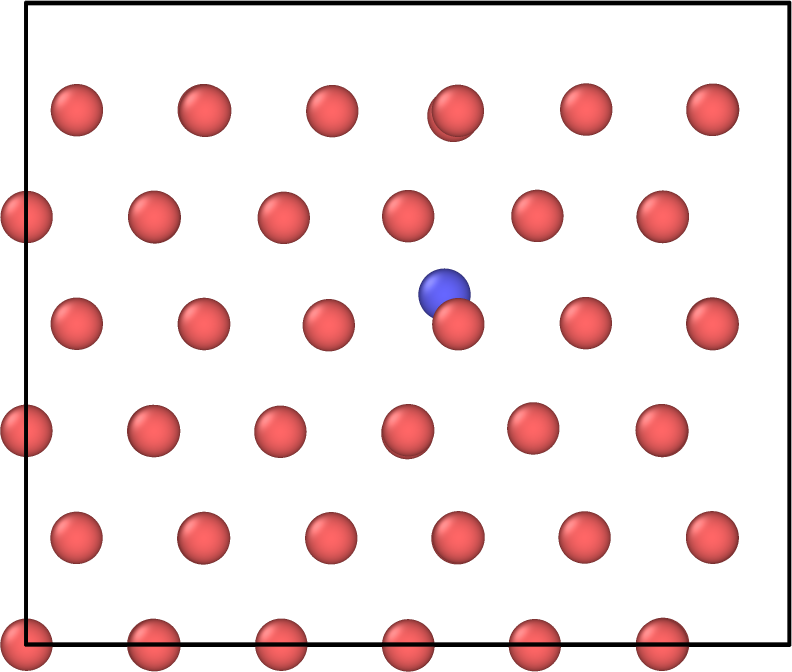
\includegraphics[width=0.8\textwidth]{ndvacz.png}
    \caption{2D projection of a slice of the relaxed structure of Nd atom inserted into $\alpha$ U as a substitutional with a nearest-neighbor vacancy (positive z axis) in the corrugated plane.  View is (100) plane.}\label{fig:ndvacz}
\end{figure}  

Nd with vac X - sits in middle of two lattice sites, as shown in Figure \ref{fig:ndvacx}.

\begin{figure}[ht]
	\centering
	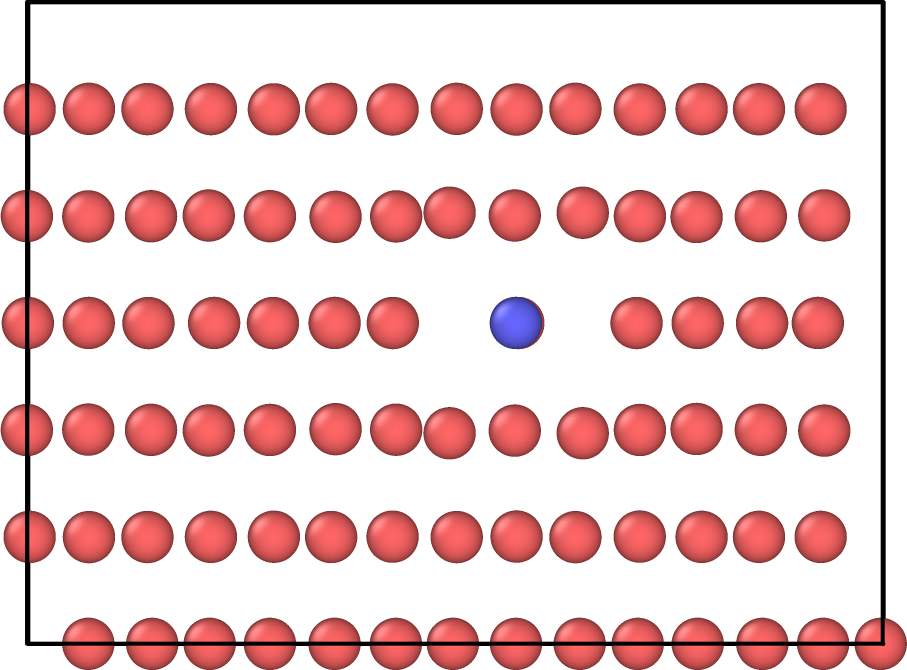
\includegraphics[width=0.8\textwidth]{ndvacx.png}
    \caption{2D projection of a slice of the relaxed structure of Nd atom inserted into $\alpha$ U as a substitutional with a nearest-neighbor vacancy (positive x axis) in the corrugated plane.  View is (010) plane.}\label{fig:ndvacx}
\end{figure}  

\begin{figure}[ht]
	\centering
	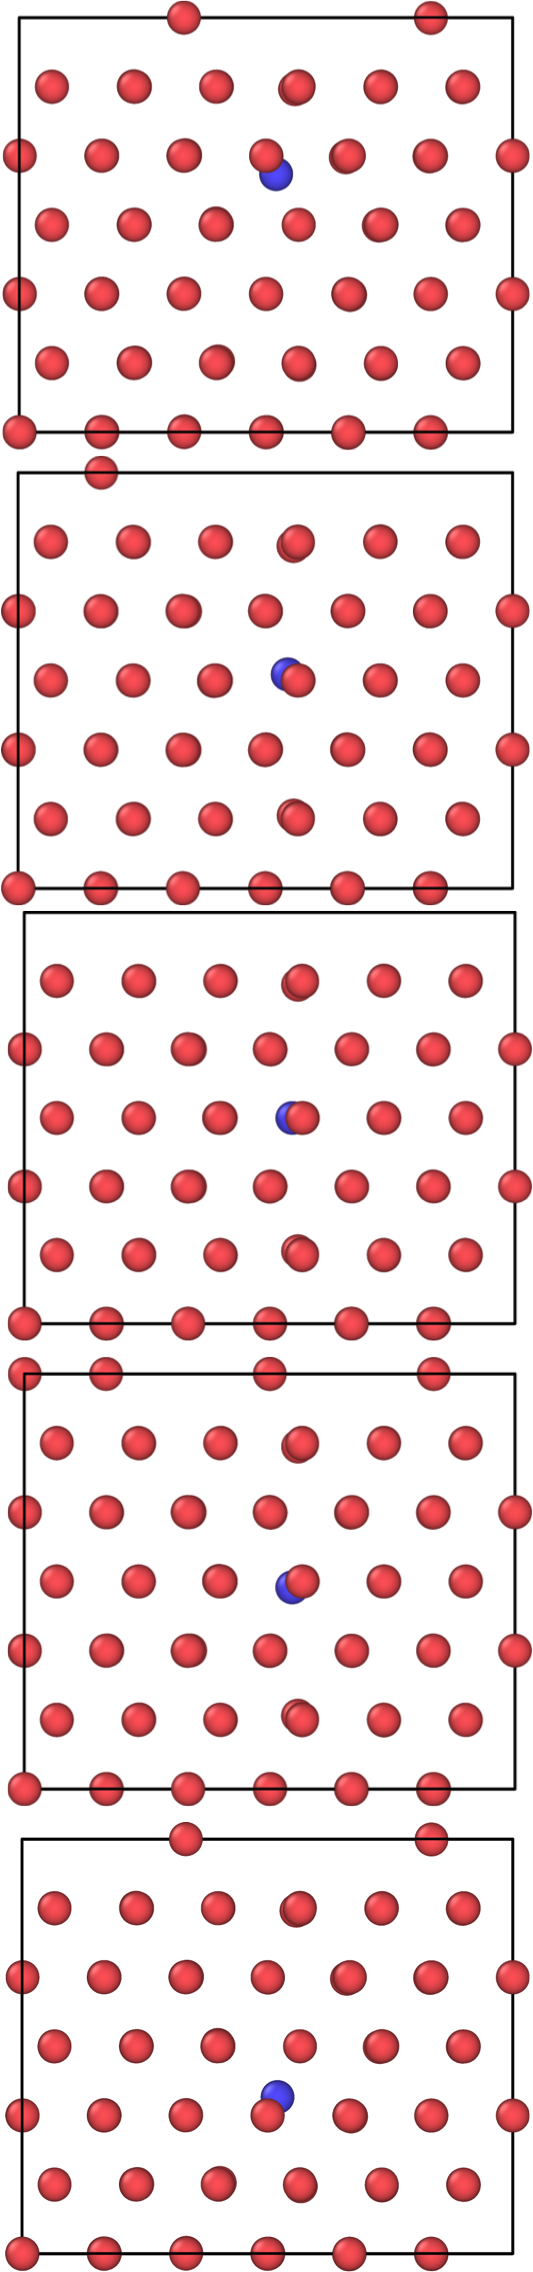
\includegraphics[width=0.3\textwidth]{nd_divac_mig.png}
    \caption{Schematic of Nd atom diffusion within a Nd-divacancy complex.}\label{fig:nd_divac_mig}
\end{figure}  


\FloatBarrier
\section{Conclusions}


\section{Acknowledgement}


\FloatBarrier

\bibliography{MARMOTbib}


\end{document}  
